\openingarticle
\def\ppages{\pagerange{ASA:firstpage}{ASA:lastpage}}
\def\shortauthor{Ülle Aguraiuja, Rachel Faulkner-Jones, Marta Lorenzon, Cindy Nelson-Viljoen}
\def\shorttitle{Third ‘Annual Student Archaeology’ Conference: Edinburgh, June 2015}
\def\maintitle{Third ‘Annual Student Archaeology’ Conference:  Edinburgh, June 2015}
\def\authormail{asa2015edinburgh@gmail.com}
\def\affiliation{School of History, Classics and Archaeology, University of Edinburgh}
%--------------------------------------------------------------
\mychapter{\maintitle}
\begin{center}
	{\Large\scshape Ülle Aguraiuja\footnote{\textit{Ülle Aguraiuja}'s research focuses on reconstructing palaeodiet and -ecology based on stable isotope analysis. She is currently working on Bronze Age skeletal material from Romania for her PhD thesis.},
		Rachel Faulkner-Jones\footnote{\textit{Rachel Faulkner-Jones}' research focuses on bronze weaponry from the Early Bronze Age in Scotland; using archival and experimental methods, it aims to better understand the function of early weaponry and the structure of EBA society in northern Europe.},\\ 
		Marta Lorenzon\footnote{\textit{Marta Lorenzon}'s interests lays on material culture and built environment. Her PhD research investigates earthen construction techniques in Bronze Age Crete domestic architecture.}, 
		Cindy Nelson-Viljoen\footnote{\textit{Cindy Nelson-Viljoen}'s PhD investigates seasonal shellfish use during the Later Stone Age of South Africa though stable isotope and sclerochronological analysis in order to better understand occupational histories of past populations, and the possible seasonal nature of their coastal diet.} }\\[1em]
	\email\\
	\affiliation
\end{center}
\vspace{3em}
\midarticle
%--------------------------------------------------------------


\label{ASA:firstpage}%


	\lettrine[nindent=0em,lines=3]{T}{he} third Annual Student Archaeology (ASA) Conference, ‘Developing Integrated Archaeology' was held at the School of History, Classics and Archaeology at the University of Edinburgh on the \nth{11}-\nth{13} June 2015. The ASA conference series, organized by and for students, was established in 2013 with the aim to offer undergraduate and postgraduate students of archaeology a constructive platform to share and discuss their research, in a relaxed, fun and engaging environment. In the last three years it has been a great experience for students to get feedback on their current research projects and to find out what other students from different universities and countries are doing. The conference was a three day event with two days of presentations, including a poster session and career roundtable discussion, followed by archaeological excursions showcasing some of Edinburgh’s heritage on the final day of the event.
	
	Oral presentations were divided into four themed sessions that tried to encompass as many fields of archaeology as possible. The session on \textit{Scientific Archaeological Methods} was intended to cover the wide field of archaeological science, including dating techniques, remote sensing and archaeological survey methods, geoarchaeology, archaeological chemistry, archaeobotany, zooarchaeology and osteological methods. The second session focused on \textit{Archaeology Beyond Academia} and included the use of methods employed in areas such as community archaeology, archaeologically themed video games and public archaeology. The third session on \textit{Applied Archaeological Theory} hosted papers on innovative interpretations of archaeological data. The papers in this session were predominantly aimed at exploring the impact of theory on the practice and analysis of artefact recovery. Finally, the \textit{Historical Archaeology} session aimed to present different case studies regarding historic cultures, which have been investigated through material culture, as well as through documented sources and oral history.
	
	The overall goal of the sessions and poster presentations was to allow students to present different research approaches to the investigation of archaeological contexts. More specifically, the conference aimed at showing and debating complementary case studies on themes such as science, theory and public outreach, and to motivate students to engage in discussion of these themes. Of the eighty students registered for ASA 2015, about half were undergraduates. The delegates were a varied group, with the number of UK students (61, 76\%) higher, than the number of foreign students (19, 24\%).
	
	The papers presented at the conference were considerably well-received not only for the quality of the research presented, but also for the variety of contexts, methodologies and topics. The first day of ASA 2015 opened with a short introduction by Professor Ian Ralston, Head of the School of History, Classics and Archaeology at the University of Edinburgh. Between the diverse and thought-provoking papers of that day, Mackenzie Downing impressed the audience with her paper \textit{An experimental investigation of sharp-force skeletal trauma with replica Bronze Age weapons}. She gave a live demonstration on how the blow was carried out and what the impact traces would be on the skeletal remains.
	
	A thought-provoking discussion ensued after Theresa O’Mahony gave her talk \textit{Archaeology for All} on archaeology and disabilities and how, often, archaeology is still not open to everyone. It was a particularly stimulating discussion based on the realization that it is our responsibility as archaeologists to ensure that archaeology, as a profession, is more accessible to both professionals and students with physical and/or invisible disabilities. Day one was closed by Professor Lord Colin Renfrew, who delivered the keynote lecture: \textit{Difficult integration. Archaeology, language and genetics: the Indo-European problem revisited}. Professor Renfrew highlighted the complications of an interdisciplinary approach in investigating archaeological data, but also the importance of it. He believed it to be the best method of breaking through and enriching the discipline with new discoveries as well as confirming an initial hypothesis.
\begin{wrapfigure}{O}{.6\textwidth}%[!htb]
	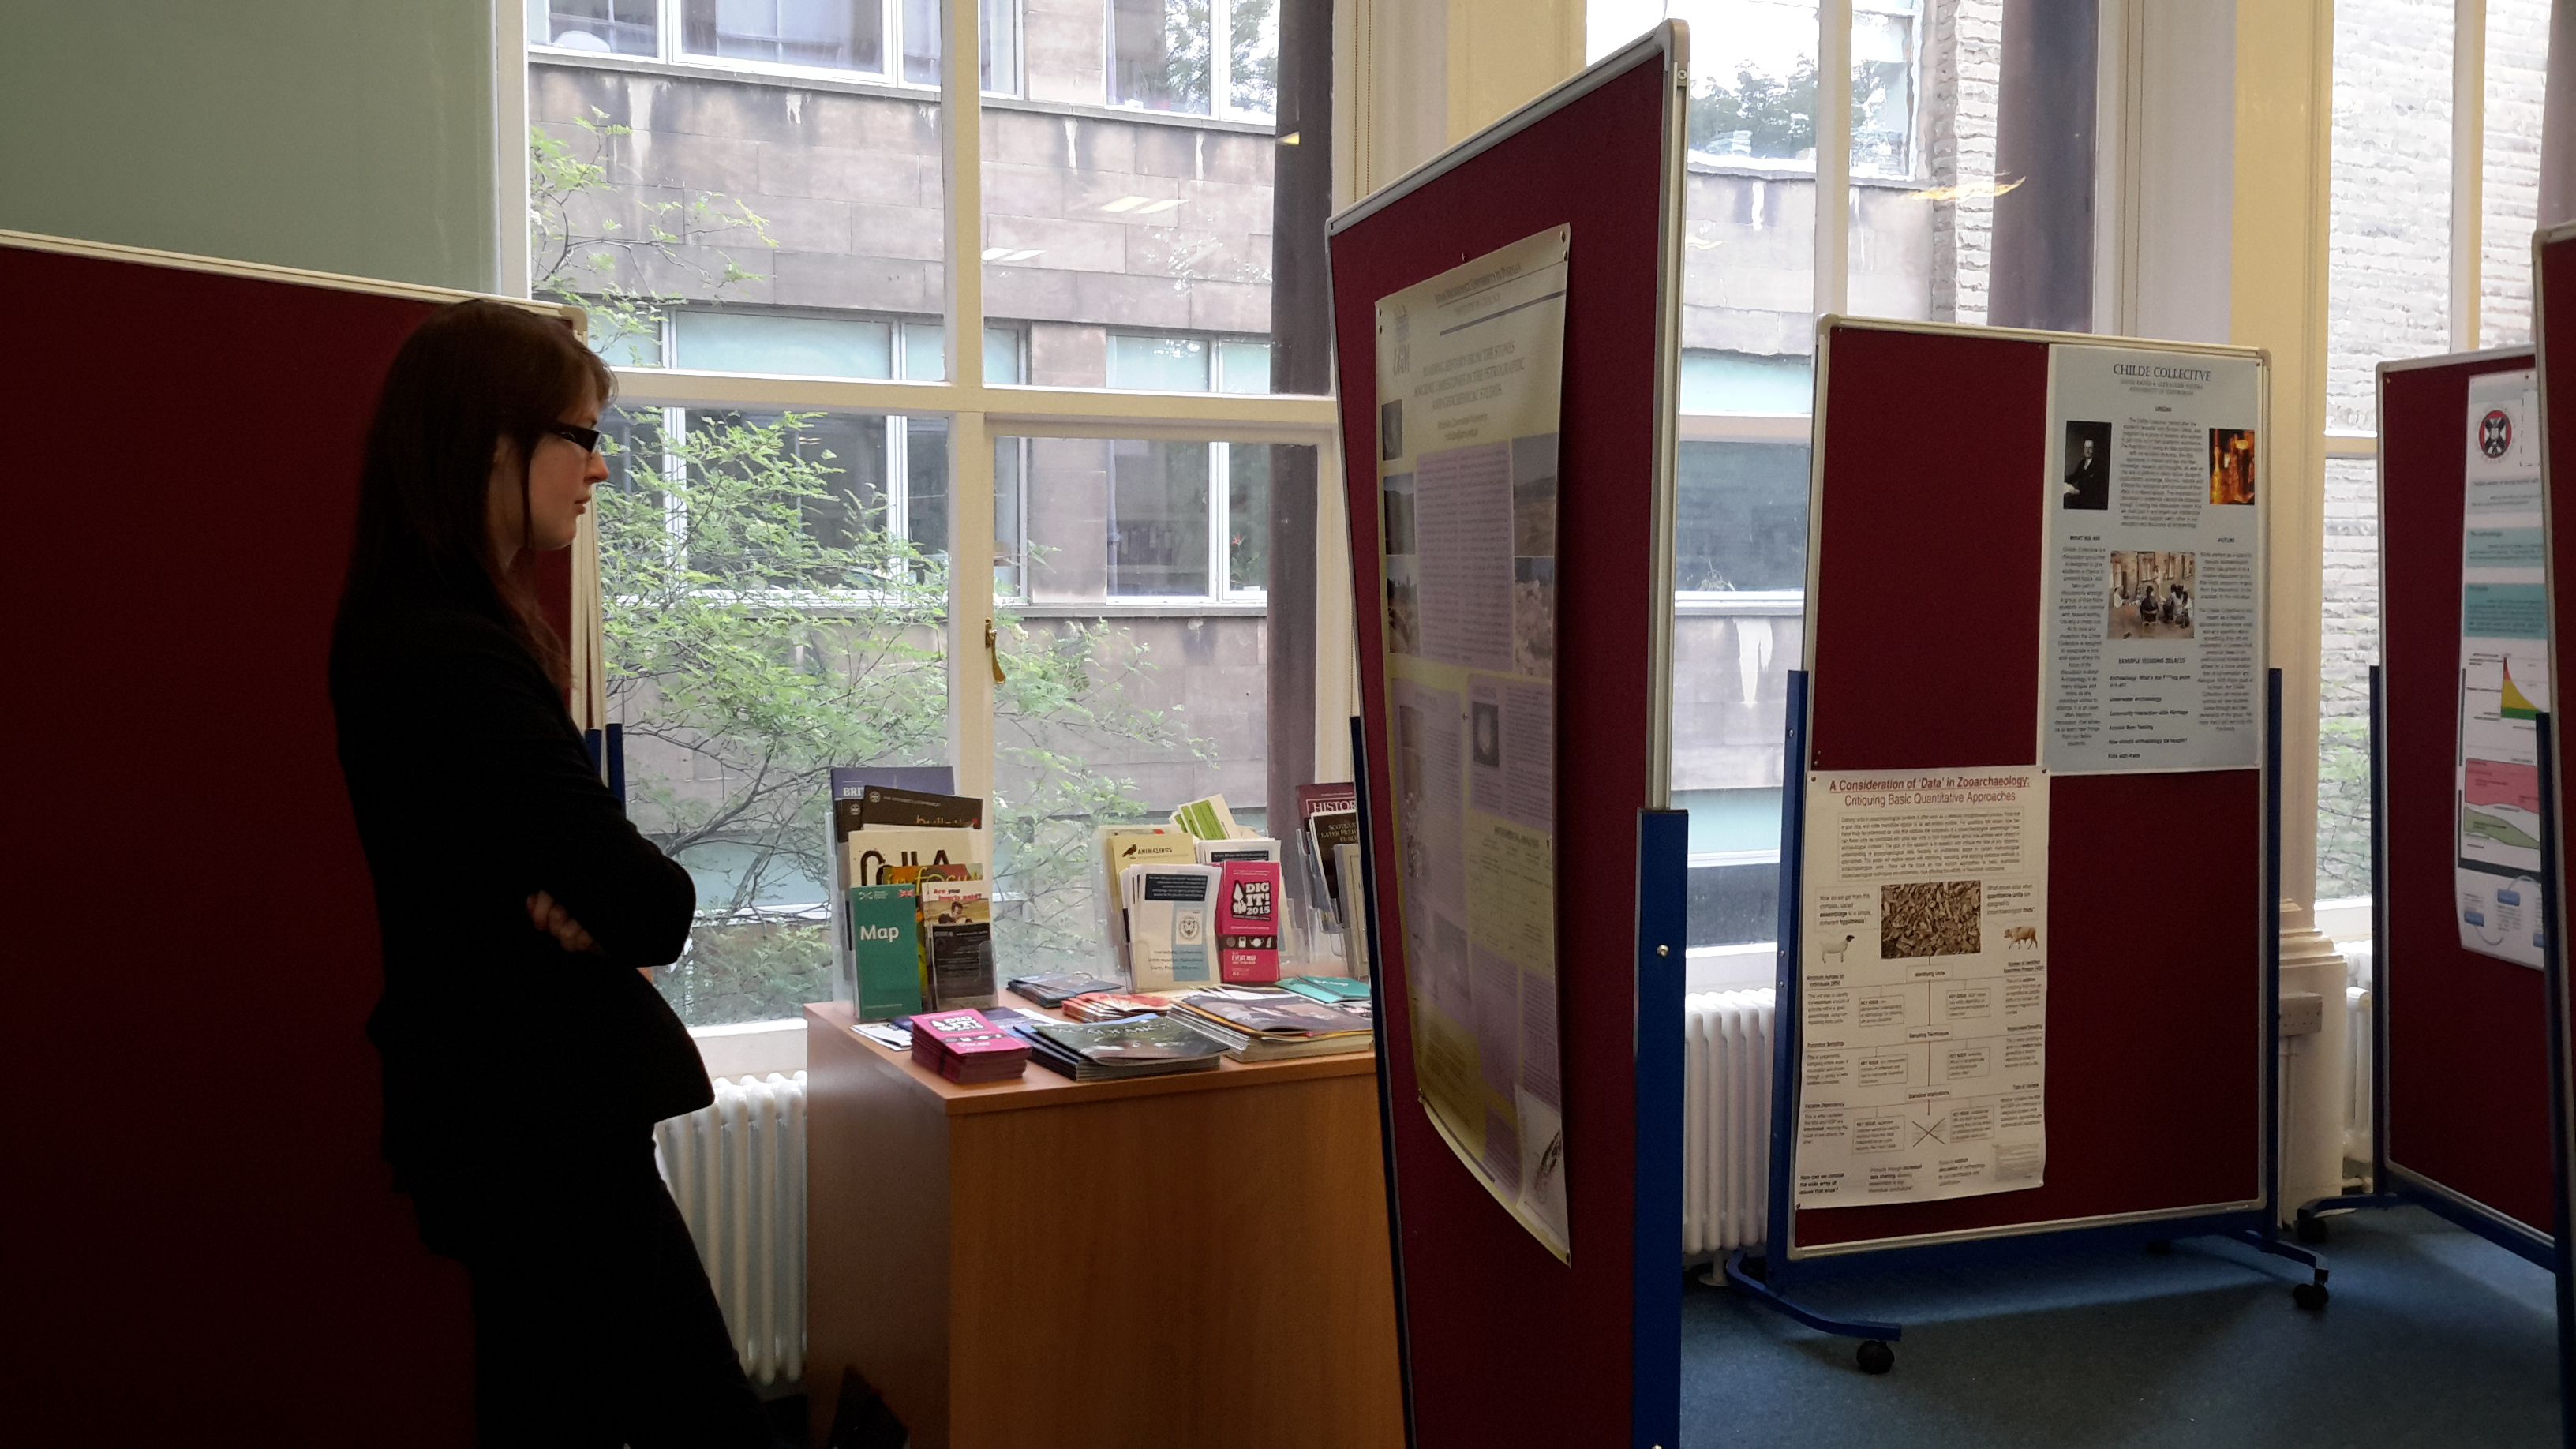
\includegraphics[width=\linewidth]{figures/ASA_Fig1}
	\centering
	\caption{Poster Session. Courtesy of ASA2015 Committee.}
	\label{fig:ASA_Fig1}
\end{wrapfigure}
	
	The second day was as inspiring as the first day with the session on Public Archaeology and Community Engagement being one of the most followed sessions both via social media and in the lecture theatre. Emily Stammitti, in particular, gave an enthusiastic presentation titled \textit{Impact above the intertidal zone} in which she focused on underwater archaeology and community engagement. The poster session (Fig. \ref{fig:ASA_Fig1}) took place during the lunch break on the second day, with the poster \textit{Archaeology of Elegy} on video-games and archaeology by Tara Copplestone winning the best poster award of the \nth{3} ASA conference, sponsored by The Society of Antiquaries of Scotland. Additional prizes were kindly offered by Historic Scotland for the best papers in each session. The winners were: Gary Pratt (\textit{Speed under sail in the Aegean MBA: Testing optimal maritime networks}), Mackenzie Downing, Emily Stammitti, and Peter Swallow (\textit{The early life of the Theatre of Dionysus at Athens}). Honorable mentions for important talks raised during the \nth{3} ASA went to Theresa O'Mahony, Mackenzie Downing, and David Banks (\textit{Community interaction with archaeological heritage: Case study from the Hagar Qim and Mnajdra temples World Heritage Site at Orendi, Malta}), who each received a colorful T-shirt sponsored by DigIt2015.
	

The second day ended with a roundtable discussion moderated by Tom Gardner on career paths in archaeology, focusing on both the academic and non-academic strands. The discussion panel consisted of Dr. Andrew Heald (AOC Archaeology), Dr. Alison Sheridan (Curator of Early Prehistory at National Museum of Scotland), David Connolly (BAJR), Gaille MacKinnon (Centre for Anatomy \& Human Identification, University of Dundee) and Dr. Simon Gilmour (Director of Society of Antiquities of Scotland). It was an amazing group of specialists from different branches of the archaeological career spectrum: commercial, museums, academia, and forensics. They helped students in answering questions about what a career in archaeology demands, and what the required skills are and how to achieve them.

\begin{wrapfigure}{O}{.6\textwidth}%[!htb]
	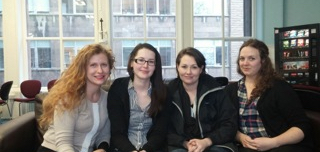
\includegraphics[width=\linewidth]{figures/ASA_Fig2}
	\caption{Organising committee (left to right): Ülle Aguraiuja, Rachel Faulkner-Jones, Marta Lorenzon, Cindy Nelson-Viljoen.}
	\label{fig:ASA_Fig2}
\end{wrapfigure}	

As organizing committee (Fig. \ref{fig:ASA_Fig2}) it was humbling for us to receive so many suitable and interesting abstracts for both the paper and poster sessions. It was a pleasure to witness the students fulfill our conference aims of organizing a platform for the sharing of ideas and useful discussions. We tried to make the conference as accessible as possible by also opening the discussion on the ASA 2015 Twitter page (\href{https://twitter.com/asa2015edin}{@ASA2015Edin}, \href{https://twitter.com/search?q=\%23asa2015\&lang=en}{\#ASA2015}) where the most relevant highlights of each paper were live tweeted as incentive for further discussions on the web as well as in the lecture theatre. In this short review it is not possible to mention all the amazing papers that have been presented, but we would like to thank all the presenters who were part of the \nth{3} ASA Conference.

	
Finally, we would like to thank everyone who made this conference possible and without whom this event would not have been successful. Special mention must be given to our sponsors: The School of History, Classics and Archaeology (University of Edinburgh), The Society of Antiquaries of Scotland, The Prehistoric Society, Dig It 2015, The Royal Archaeological Institute, Centre for Medieval and Renaissance Studies (University of Edinburgh), Historic Scotland, Edinburgh University Archaeology Society and the volunteers from the University of Edinburgh who helped us during the day.
\label{ASA:lastpage}
%----------------------------------------------------------------------------------------
\closingarticle
\endinput
